\documentclass[12pt,letterpaper]{article}
\usepackage[utf8]{inputenc}
\usepackage{amsmath}
\usepackage{amsfonts}
\usepackage{amssymb}
\usepackage{graphicx}
\usepackage[left=2cm,right=2cm,top=2cm,bottom=2cm]{geometry}
\author{Kris Garrett}
\title{Tycho 2 User Guide (Draft)}
\begin{document}
\maketitle


\section{Introduction}
Tycho 2 is a reworking of a code named Tycho written by Shawn Pautz around the year 2000.
The original code solved a linear, kinetic, transport equation on an unstructured, 3D tetrahedral mesh and was parallelized via MPI.
The original code was made to test the performance of transport sweeps which will be subsequently described.

Tycho 2 solves the same equation with some additions.
The new code adds energy dependence to the calculations to give realistic computational results for cases with several energy groups.
The code is implemented in MPI and OpenMP and uses only open source software and libraries to generate meshes and compile.


\section{The equation}
Tycho 2 solves the following kinetic equation with isotropic scattering
\begin{equation} \label{eq:main}
\Omega \cdot \nabla_x \Psi(x,\Omega,E) + \sigma_t \Psi(x,\Omega,E) = \frac{\sigma_s}{4\pi} \int_{\mathbb{S}^2} \Psi(x,\Omega',E) d\Omega' + Q(x,\Omega,E).
\end{equation}
The function $\Psi$ is the unknown, $\sigma_t$ and $\sigma_s$ are the total and scattering cross sections with $\sigma_t > \sigma_s$ and are constant.
The function $Q$ is a known source.

The independent variables are:
\begin{itemize}
\item Space -- $x \in \mathcal{D} \subset \mathbb{R}^3$,
\item Direction -- $\Omega \in \mathbb{S}^2$ (the unit sphere), 
\item Energy -- $E \in \mathbb{R}^{\geq 0}$.
\end{itemize}
Notice the equation is dependent on energy, but the different energies are not coupled.
This is done on purpose since the goal is to test sweeping strategies which are uncoupled in energy.

For the purpose of simpler notation, define
\begin{equation}
\Phi(x,E) = \int_{\mathbb{S}^2} \Psi(x,\Omega',E) d\Omega'
\end{equation}
to get the equivalent equation
\begin{equation} \label{eq:main1}
\Omega \cdot \nabla_x \Psi(x,\Omega,E) + \sigma_t \Psi(x,\Omega,E) = \frac{\sigma_s}{4\pi} \Phi(x,E) + Q(x,\Omega,E).
\end{equation}


\section{Method of discretization}
Equation \eqref{eq:main1} is discretized using: discontinuous Galerkin (DG) with linear elements in $x$, discrete ordinates in $\Omega$, and energy groups in $E$.

\paragraph{Energy discretization.}
Since equation~\eqref{eq:main1} is not coupled in energy, the discretization of $E$ does not matter.
Hence, $E$ discretized in energy will be denoted by $E_g$ where $g$ is an integer indexing in energy group.
The input deck for Tycho 2 allows the user to set the number of energy groups $G$.

\paragraph{Angle discretization.}
As stated, angle is discretized via discrete ordinates, which is often denoted as S$_N$ where $N$ is the order of the discretization.
Tycho 2 implements the Chebyshev-Legendre quadrature of the sphere.

Given the parameterization $(\mu,\theta)$ of the sphere where $\mu$ is on the z-axis and $\theta$ is the angle in the plane $z = \mu$, the Chebyshev-Legendre quadrature is given by weights $w_q$ and nodes $\Omega_q = (\mu_{q_1}, \theta_{q_2})$.
The indices have ranges $q = 0, \ldots, 2N^2-1$, $q_1 = 0, \ldots, N-1$, and $q_2 = 0, \ldots, 2N-1$.
The node is discretized as $\mu$ along $N$ Legendre nodes and $\theta$ along $2N$ equally spaced angles in $[0,2\pi]$.
The weights are scaled Legendre weights so that $\sum_q w_q = 4 \pi$.

\paragraph{Spatial discretization.}
Space is discretized via DG.
In each tetrahedral cell $C_i$, define basis functions $b_{ik}|_{k=0}^3$ to be linear interpolation functions with 
\begin{equation}
b_{ik} = \begin{cases}
1, \textrm{ at vertex } k \textrm{ of cell } C_i \\
0, \textrm{ at other vertices of cell } C_i
\end{cases}.
\end{equation}

Define 
\begin{equation}
\Psi|_{C_i} = \sum_k \Psi_{ik} b_k.
\end{equation}

\begin{align*}
\frac{1}{12} \bar{A}_1 \left( 2\hat{\Psi}^{(1)}_0 + \hat{\Psi}^{(1)}_2 + \hat{\Psi}^{(1)}_3 \right)
+ \frac{1}{12} \bar{A}_2 \left( 2\hat{\Psi}^{(2)}_0 + \hat{\Psi}^{(2)}_1 + \hat{\Psi}^{(2)}_3 \right)
+ \frac{1}{12} \bar{A}_3 \left( 2\hat{\Psi}^{(3)}_0 + \hat{\Psi}^{(3)}_1 + \hat{\Psi}^{(3)}_2 \right) \\
+ \frac{1}{12} \bar{A}_0 \left( \Psi_0 + \Psi_1 + \Psi_2 + \Psi_3 \right)
+ \frac{\sigma_t V}{20} \left( 2\Psi_0 + \Psi_1 + \Psi_2 + \Psi_3 \right)
= \frac{V}{20} \left( 2Q_0 + Q_1 + Q_2 + Q_3 \right)
\end{align*}
\begin{align*}
\frac{1}{12} \bar{A}_0 \left( 2\hat{\Psi}^{(1)}_1 + \hat{\Psi}^{(1)}_2 + \hat{\Psi}^{(1)}_3 \right)
+ \frac{1}{12} \bar{A}_2 \left( \hat{\Psi}^{(2)}_0 + 2\hat{\Psi}^{(2)}_1 + \hat{\Psi}^{(2)}_3 \right)
+ \frac{1}{12} \bar{A}_3 \left( \hat{\Psi}^{(3)}_0 + 2\hat{\Psi}^{(3)}_1 + \hat{\Psi}^{(3)}_2 \right) \\
+ \frac{1}{12} \bar{A}_1 \left( \Psi_0 + \Psi_1 + \Psi_2 + \Psi_3 \right)
+ \frac{\sigma_t V}{20} \left( \Psi_0 + 2\Psi_1 + \Psi_2 + \Psi_3 \right)
= \frac{V}{20} \left( Q_0 + 2Q_1 + Q_2 + Q_3 \right)
\end{align*}
\begin{align*}
\frac{1}{12} \bar{A}_0 \left( \hat{\Psi}^{(1)}_1 + 2\hat{\Psi}^{(1)}_2 + \hat{\Psi}^{(1)}_3 \right)
+ \frac{1}{12} \bar{A}_1 \left( \hat{\Psi}^{(2)}_0 + 2\hat{\Psi}^{(2)}_2 + \hat{\Psi}^{(2)}_3 \right)
+ \frac{1}{12} \bar{A}_3 \left( \hat{\Psi}^{(3)}_0 + \hat{\Psi}^{(3)}_1 + 2\hat{\Psi}^{(3)}_2 \right) \\
+ \frac{1}{12} \bar{A}_2 \left( \Psi_0 + \Psi_1 + \Psi_2 + \Psi_3 \right)
+ \frac{\sigma_t V}{20} \left( \Psi_0 + \Psi_1 + 2\Psi_2 + \Psi_3 \right)
= \frac{V}{20} \left( Q_0 + Q_1 + 2Q_2 + Q_3 \right)
\end{align*}
\begin{align*}
\frac{1}{12} \bar{A}_0 \left( \hat{\Psi}^{(1)}_1 + \hat{\Psi}^{(1)}_2 + 2\hat{\Psi}^{(1)}_3 \right)
+ \frac{1}{12} \bar{A}_1 \left( \hat{\Psi}^{(2)}_0 + \hat{\Psi}^{(2)}_2 + 2\hat{\Psi}^{(2)}_3 \right)
+ \frac{1}{12} \bar{A}_2 \left( \hat{\Psi}^{(3)}_0 + \hat{\Psi}^{(3)}_1 + 2\hat{\Psi}^{(3)}_3 \right) \\
+ \frac{1}{12} \bar{A}_3 \left( \Psi_0 + \Psi_1 + \Psi_2 + \Psi_3 \right)
+ \frac{\sigma_t V}{20} \left( \Psi_0 + \Psi_1 + \Psi_2 + 2\Psi_3 \right)
= \frac{V}{20} \left( Q_0 + Q_1 + Q_2 + 2Q_3 \right)
\end{align*}


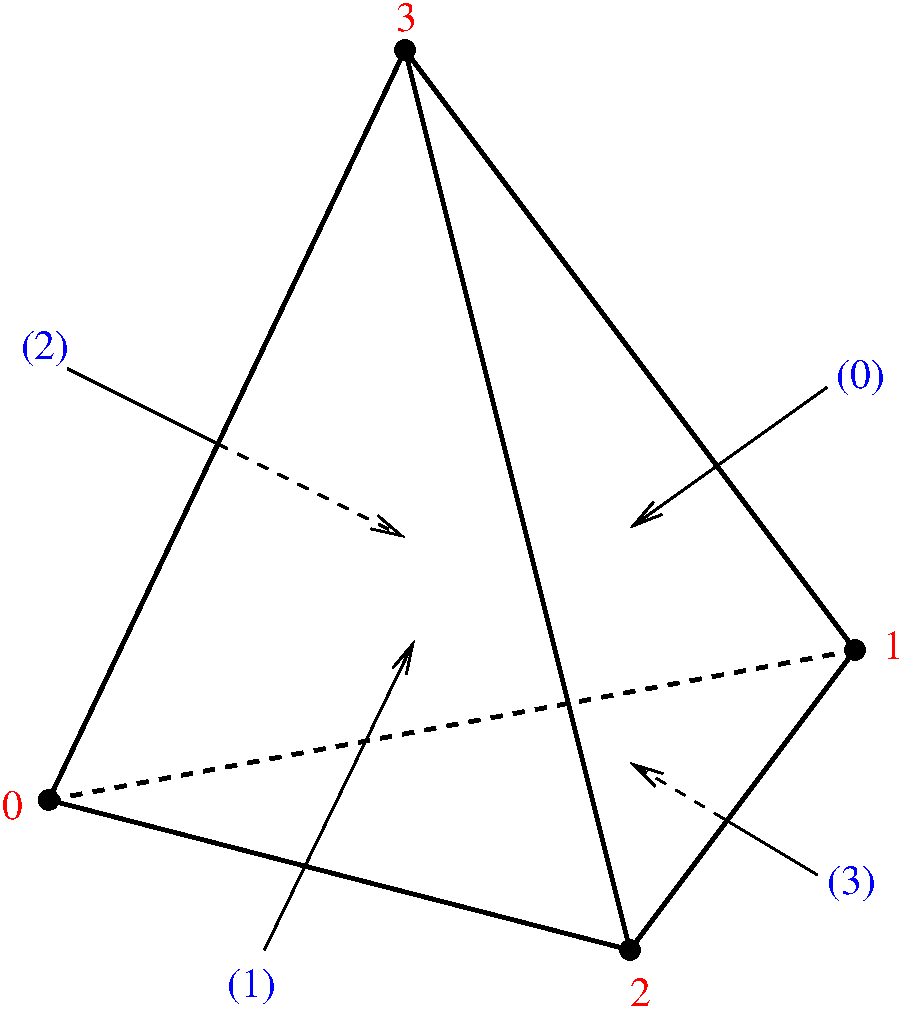
\includegraphics[scale=0.5]{tet-eps-converted-to.pdf}







\end{document}